\documentclass{article} % \documentclass{} is the first command in any LaTeX code.  It is used to define what kind of document you are creating such as an article or a book, and begins the document preamble

\usepackage{amsmath} % \usepackage is a command that allows you to add functionality to your LaTeX code
\usepackage{graphicx}
\graphicspath{ {./images/} }
\title{Discrete Time Signals and Systems} % Sets article title
\author{Hunter Mills} % Sets authors name
\date{\today} % Sets date for date compiled

% The preamble ends with the command \begin{document}
\begin{document} % All begin commands must be paired with an end command somewhere
    \maketitle % creates title using information in preamble (title, author, date)
    
    \section{Frequency Domain Analysis of LTI Systems} % creates a section
    These notes only cover 5.1, 5.2.1 and 5.4.1.
    
    This chapter investigates the characterization of LTI systems in the frequency domain. The excitation signals in this chapter are mostly complex exponential's and sinusoidal functions. 
    \subsection{Frequency Domain Characteristics of LIT Systems}
    The characterization of the LTI systems are described with the frequency variable $\omega$ called the frequency response $H(\omega)$. The frequency response function completely characterizes a LTI system in the frequency domain. This allows us to determine the steady state response of the system to any arbitrary weighted linear combination of sinusoidal or complex exponentials. \\
    \textbf{Response to Complex Exponential and Sinusoidal Signals}\\
    
    The response and any relaxed LTI system to x(n) is given by the convolution sum
	\begin{equation}
	y(n) = \sum_{k=-\infty}^{\infty} h(k)x(n-k)
	\end{equation}
	This system is excited with 
	\begin{equation}
	x(n) = Ae^{j\omega n}, \;\;\; -\infty<n<\infty
	\end{equation}
	When substituting that into the convolution sum, the response is
	\begin{equation}
	y(n) = \sum_{k=-\infty}^{\infty} h(k)[Ae^{-j\omega (n-k)}]
	\end{equation}
	\begin{equation}
	y(n) = A[\sum_{k=-\infty}^{\infty} h(k)e^{-j\omega k}]e^{j\omega n}
	\end{equation}
	The term in the brackets above is a function of $\omega$ and is the Fourier Transform of the unit sample response $h(k)$ of the system. Hence,
	\begin{equation}
	H(\omega) = \sum_{k=-\infty}^{\infty}h(k)e^{-j\omega k}
	\end{equation}
	The response of the system to the complex exponential is 
	\begin{equation}
	y(n) = AH(\omega)e^{-j\omega n}
	\end{equation}
	The response to a complex exponential is a complex exponential with the same frequency as the input but scaled by $H(\omega)$. This is an \textit{eigenfunction}, a function that when used as an input to a system produces an output of the same frequency scaled by a factor and phase shifted. Since $H(\omega)$ is the Fourier transform of h(k), we can calculate it by
	\begin{equation}
	h(k) = \frac{1}{2\pi} \int_{-\pi}^{\pi}H(\omega)e^{j\omega k} d\omega
	\end{equation}
	For a LTI system with a real-valued impulse response, the magnitude and phase have the following symmetry properties.
	\begin{equation}
	H_R(\omega) = \sum_k h(k)\cos \omega k
	\end{equation}
	\begin{equation}
	H_I(\omega) = -\sum_k h(k)\sin \omega k
	\end{equation}
	\begin{equation}
	|H(\omega)| = \sqrt{H_R^2 (\omega) + H_I^2(\omega)}
	\end{equation}
	\begin{equation}
	\Theta (\omega) = \arctan(\frac{H_I (\omega)}{H_R (\omega)})
	\end{equation}
	$H_R(\omega)$ is even and $H_I(\omega)$ is odd in reference to $\omega$. 
	
	In the most general case, if the input to the system consists of an arbitrary linear combination of sinusoids of the form
	\begin{equation}
	x(n) = \sum_{i=1}^{L}A_i \cos (\omega_i n + \phi_i), \;\;\; -\infty < n < \infty
	\end{equation}
	where $A_i$ and $\phi_i$ are the amplitudes and phases of the corresponding sinusoidal components, then the response of the system is
	\begin{equation}
	y(n) = \sum_{i=1}^{L}A_i |H(\omega_i)|\cos[\omega_i n + \phi_i + \Theta (\omega_i)]
	\end{equation}
	We can view that LTI systems act as a filter to sinusoids.  \\
	\textbf{Steady State and Transient Response to Sinusoidal Input Signal}\\
	
	In the previous section we looked at the response of a LTI system when the input was applied to the system at $n=-\infty$. This is the steady state response, in this section we will look the transient response, when the input is applied at some finite time instant (ie n=0). The response of the system has two terms, the steady state and the transient. To demonstrate, here is an example, a system described by the first order difference equation
	\begin{equation}
	y(n) = ay(n-1) + x(n)
	\end{equation}
	This is calculated by plugging in $n=0,1,2...$ and simplifying the equation. The response to any input applied at $x(n)$ is shown below. 
	\begin{equation}
	y(n) = a^{n+1}y(-1) + \sum_{k=0}^{n}a^kx(n-k)
	\end{equation}
	where $y(-1)$ is the initial condition. Assume the input is
	\begin{equation}
	x(n) = Ae^{j\omega n}, \;\;\; n \ge 0
	\end{equation}
	When we substitute the previous equation into $y(n)$ we get
	\begin{equation}
	y(n) = a^{n+1}y(-1)+A\sum_{k=0}^n a^ke^{j\omega n}
	\end{equation}
	\begin{equation}
	y(n) = a^{n+1}y(-1)+A[\sum_{k=0}^n (ae^{-j\omega})^k]e^{j\omega n}
	\end{equation}
	\begin{equation}
	y(n) = a^{n+1}y(-1) + A\frac{1-a^{n+1}e^{-j\omega (n+1)}}{1-ae^{-j\omega}e^{j\omega n}}
	\end{equation}
	\begin{equation}
	y(n) = a^{n+1}y(-1)+ \frac{Aa^{n+1}e^{-j\omega (n+1)}}{1-ae^{-j\omega}e^{-j\omega n}} + \frac{A}{1-ae^{-j\omega}}e^{-j\omega n}
	\end{equation}
	The steady state response is calculated by taking the limit of $y(n)$ as $n \rightarrow \infty$. The transient response is the first two terms in $y(n)$. The first term is the zero-input response and the second term is produced by the exponential input signal.\\
	\textbf{Steady-State Response to Periodic Input Signals}\\
	
	Suppose the input to a stable LTI system is a periodic signal with period N. Since such a signal exists from $-\infty < n < \infty$, the response of the system at any time instant $n$ is equal to the steady state response. The response of the system to a periodic input signal is also periodic with the same period N. \\
	\textbf{Response to Aperiodic Input Signals}\\
	When the input signal is aperiodic, we can use the Fourier transform to calculate $X(\omega)$ and $H(\omega)$. The convolution theory is used to calculate the response of the system
	\begin{equation}
	Y(\omega) = X(\omega)H(\omega)
	\end{equation}
	One of the most important relationships is
	\begin{equation}
	H(\omega) = \frac{Y(\omega)}{H(\omega)}
	\end{equation}
	
	\begin{figure}[h]
	\centering
	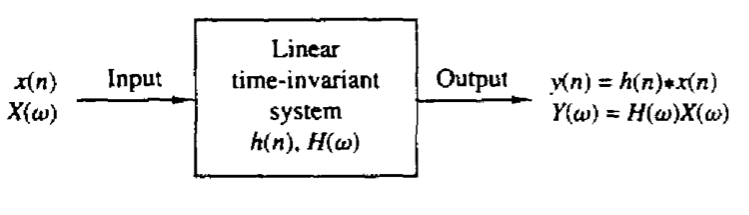
\includegraphics[width=10cm]{conv_lti}
	\caption{Input output relationships for LTI systems}
	\end{figure}
	\subsection{Frequency Response of LTI Systems}
	In this section we focus on determining the frequency response of LTI systems that have rational system functions. This call of LTI systems is described in the time domain by constant-coefficient difference equations.\\
	\textbf{Frequency Response of a System with a Rational System Function}\\
	
	If a system function $H(z)$ converges on the unit circle we can obtain the frequency response by evaluating $H(z)$ on the unit circle. 
	\begin{equation}
	H(\omega) = H(z)|_{z=e^{j\omega}} = \sum_n h(n)e^{-j\omega n}
	\end{equation}
	When $H(z)$ is a rational function we have
	\begin{equation}
	H(\omega) = \frac{B(\omega)}{A(\omega)} = \frac{\sum_{k=0}^M b_ke^{-j\omega k}}{1 + \sum_{k=1}^N a_k e^{-j\omega k}}
	\end{equation}
	and
	\begin{equation}
	y(n) = b_0 \frac{\Pi_{k=1}^M (1-z_ke^{-j\omega})}{\Pi_{k=1}^N (1-p_ke^{-j\omega})}
	\end{equation}
	where $a_k and b_k$ are real but $z_k and p_k$ may be complex. Sometimes we want to express $H(\omega)$ as $H(z)$ where 
	\begin{equation}
	|H(\omega)|^2 = H(\omega)H^*(\omega)
	\end{equation}
	$H(\omega)$ is obtained by evaluating $H^*(1/z^*)$. When $h(n)$ is real then the correlation table of the z-transform says $H(z)H(z^{-1})$ is the z-transform of the autocorrelation sequence $r_{hh}(m)$ of the unit sample response $h(n)$. The Wiener-Khintchine theorem states that $|H(\omega)|^2 = \mathcal{F}[r_{hh}(m)]$. If $H(z) = B(z)/A(z)$ the transforms $D(z)=B(z)B(z^{-1})$ and  $C(z)=A(z)A(z^{-1})$ are the z-transforms of the autocorrelation sequences $c_k$ and $d_k$. 
	\begin{equation}
	c_l = \sum_{k=0}^{N-|l|}a_ka_{k+1}, \;\;\; -N \le l \le N
	\end{equation}
	\begin{equation}
	d_l = \sum_{k=0}^{M-|l|}b_kb_{k+1}, \;\;\; -M \le l \le M
	\end{equation}
	\begin{equation}
	|H(\omega)|^2 = \frac{d_0 + 2\sum_{k=1}^M d_k \cos k\omega}{c_0 + 2\sum_{k=1}^M c_k \cos k\omega}
	\end{equation}
	and $\cos k\omega$ can be expressed as a polynomial function of $\cos \omega$
	\begin{equation}
	\cos k\omega = \sum_{m=0}^k \beta_m (\cos \omega)^m
	\end{equation}
	where $\beta_m$ are the coefficients in the expansion. While it is easy to determine $H(z^{-1})$ given $H(z)$ but is not easy to calculate $H(z)$ given $h(n)$
	
	\subsection{LTI Systems as Frequency-Selective Filters}
	A LTI system performs a type of filtering among the various frequency components at its input. The nature of the filtering action is determined by the frequency response characteristics $H(\omega)$. \\
	\textbf{Ideal Filter Characteristics}\\
	
	Filters are classified according to their frequency domain characteristics as low, high, bandpass, bandstop or band elimination filters. The ideal magnitude response of these filters is shown in the figure below. An ideal filter has constant gain in the passband and zero gain in the stopband. Another characteristic is the linear phase response.
	\begin{equation}
	H(\omega) = 
		\begin{cases}
      	Ce^{-j\omega n_0}, & \;\;\; \omega_1 < \omega < \omega_2 \\
      	0, & \text{otherwise}
    	\end{cases} 
	\end{equation}
	The frequency response is shown as 
	\begin{equation}
	Y(\omega) = X(\omega)H(\omega)
	\end{equation}
	\begin{equation}
	Y(\omega) = CX(\omega)e^{-j\omega n_0}
	\end{equation}
	and by applying the scaling and time shifting properties we calculate
	\begin{equation}
	y(n) = Cx(n-n_0)
	\end{equation}
	The ideal filters have a linear phase characteristic in their passband
	\begin{equation}
	\Theta(\omega) = -\omega n_0
	\end{equation}
	The derivative of the phase with respect to frequency has the units of delay and the signal delay is
	\begin{equation}
	\tau_g (\omega) = -\frac{d\Theta(\omega)}{d\omega}
	\end{equation}
	$\tau_g$ is usually called the \textit{envelope delayor} or the \textit{group delay} and it is the time delay that a signal component of frequency $\omega$ undergoes as it passes from the input of the system to the output. When the phase response is linear $\tau_g (\omega) = n_0 = $ constant. The ideal low pass filter is the sinc function, but since it is not causal and not absolutely sumable it is physically unrealizable. 

	\begin{figure}[h]
	\centering
	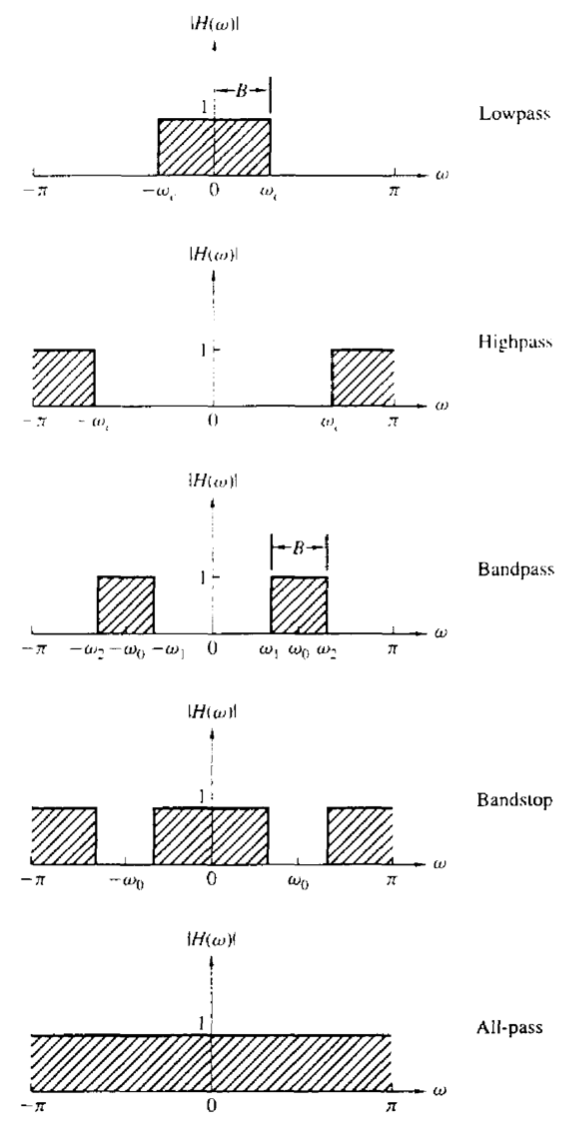
\includegraphics[width=10cm]{filt_t}
	\caption{Ideal Filter Representations}
	\end{figure}

\end{document} % This is the end of the document